\chapter{Directed graphs}\label{digraphs_chap}

\section{Digraphs}\label{digraphs_sec}

\hyperdef{directed}{graph}{A \term{directed graph}} (\term{digraph} for
short) is formally the same as a binary relation, $R$, on a set, $A$, but
we picture the digraph geometrically by representing elements of $A$ as
points on the plane, with an arrow from the point for $a$ to the point for
$b$ exactly when $(a,b) \in \graph{R}$.  The elements of $A$ are referred
to as the \emph{vertices} of the digraph, and the pairs $(a,b) \in
\graph{R}$ are called its \term{directed edges}.  We use the notation
$\diredge{a}{b}$ as an alternative notation for the pair $(a,b)$.

For example, the divisibility relation on $\set{1,2,\dots,12}$ is
represented by the digraph:
\begin{figure}[h]
\centering 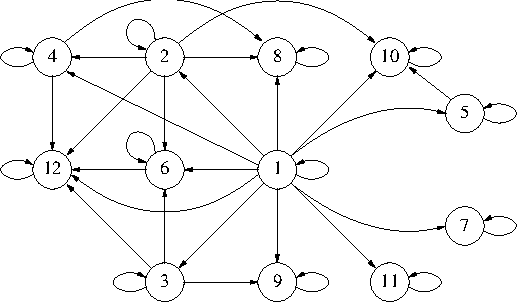
\includegraphics{figures/divisibility.pdf}
\caption{The Digraph for Divisibility on $\set{1,2,\dots,12}$.}
\label{fig:divisibility-digraph}
\end{figure}

%\hfill
%\includegraphics{divi2.pdf}
%{figures/divide12.mps}

\subsection{Paths in Digraphs}\label{paths}

Pictured with points and arrows, a length $k$ path in a digraph looks
like a line that starts at a point, $a_0$, and traverses $k$ arrows
between successive points, $a_1,a_2,\dots$ to end at a point, $a_k$.
A path is \term{simple} when it doesn't cross itself.  Here's the
precise definition:

\begin{definition}
A \emph{path in a digraph} is a sequence of vertices $a_0,\dots,a_k$
with $k \ge 0$ such that $\diredge{a_i}{a_{i+1}}$ is an edge of the
digraph for $i = 0,1,\dots, k-1$.  The path is said to \emph{start} at
$a_0$, to \emph{end} at $a_k$, and the \emph{length} of the path is
defined to be $k$.  The path is \emph{simple} iff all the $a_i$'s are
different, that is, $a_i = a_j$ only if $i=j$.
\end{definition}
Note a single vertex counts as length zero path that begins and ends
at itself.

Many of the relational properties have geometric descriptions in terms of
digraphs.  For example:
\begin{description}

\item[Reflexivity:] All vertices have self-loops (a \emph{self-loop} at a
vertex is an arrow going from the vertex back to itself).

\item[Irreflexivity:] No vertices have self-loops.

\item[Asymmetry:] No self-loops and at most one (directed) edge between
any two vertices.

\item[Symmetry:] A binary relation $R$ is
\hyperdef{graphs}{symmetric}{\term{symmetric}} iff $aRb$ implies $bRa$ for
all $a,b$ in the domain of $R$.  So if there is an edge from $a$ to $b$,
there is also one in the reverse direction.  So edges may as well be
represented without arrows, indicating that they can be followed in either
direction.

\item[Transitivity:] Short-circuits---for any path through the graph,
there is an arrow from the first vertex to the last vertex on the path.
\end{description}

We can define some new relations based on paths.  Let $R$ be the edge
relation of a digraph.  Define relations $R^*$ and $R^+$ on the vertices
by the conditions that for all vertices $a,b$:
\begin{eqnarray*}
a\, R^*\, b &\eqdef& \mbox{there is a path in $R$ from $a$ to $b$},\\
a\, R^+\, b &\eqdef& \mbox{there is a positive length path in $R$ from $a$ to $b$}.
\end{eqnarray*}

$R^*$ is called the \emph{path relation}\footnote{In many texts, $R^*$ is
called the \emph{transitive closure} of $R$.} of $R$.  It follows from the
definition of path that $R^*$ is transitive.  It is also reflexive
(because of the length-zero paths) and it contains the graph of $R$
(because of the length-one paths).  $R^+$ is called the
\emph{positive-length path relation}; it also contains $\graph{R}$ and is
transitive.

\subsection{Composition of Relations}\label{relation_compose_subsec}

There is a simple way to extend \idx{composition} of functions to
composition of relations, and this gives another way to talk about
paths in digraphs.

Let $R: B\to C$ and $S: A \to B$ be relations.  Then the
\idx{composition} of $R$ with $S$ is the binary relation $(R \compose
S): A\to C$ defined by the rule
\[
a \mrel{(R \compose S)} c \eqdef\ \exists b \in B.\, (b \mrel{R} c)
\QAND (a \mrel{S} b).
\]
This agrees with the Definition~\ref{func_compose_def} of composition
in the special case when $R$ and $S$ are functions.
\iffalse
\footnote{Some texts define $R \compose S$ the other way around, that
  is, with $S$ applied to the result of applying $R$ first.}
\fi

Now when $R$ is a digraph, it makes sense to compose $R$ with itself.
Then if we let $R^n$ denote the composition of $R$ with itself $n$
times, it's easy to check that $R^n$ is the length-$n$ path relation:
\[
a  \mrel{R^n} b \qiff \mbox{ there is a length $n$ path in $R$ from $a$ to $b$}.
\]
This even works for $n=0$, if we adopt the convention that $R^0$ is the
identity relation $\ident{A}$ on the set, $A$, of vertices.  That is, $a
\mrel{\ident{A}} b$ iff $a = b$.

\subsection{Directed Acyclic Graphs}\label{sec:dag}

\begin{definition}
A \term{cycle} in a digraph is defined by a path that begins and ends
at the same vertex.  Note that by convention, a single vertex is
considered to be a cycle of length 0 that begins and ends at the
vertex.  A \term{directed acyclic graph (DAG)} is a directed graph
with no positive length cycles.

A \term{simple cycle} in a digraph is a cycle whose vertices are distinct
except for the beginning and end vertices.
\end{definition}

\iffalse
In contrast to undirected graphs, a single vertex \emph{is} considered to
be a simple cycle.
\fi

DAG's are an economical way to represent partial orders.  For example, the
\emph{direct prerequisite} relation between MIT subjects in
Chapter~\ref{partial-order-chapter} was used to determine the partial
order of indirect prerequisites on subjects.  This indirect prerequisite
partial order is precisely the positive length path relation of the direct
prerequisites.

\begin{lemma}
If $D$ is a DAG, then $D^+$ is a strict partial order.
\end{lemma}

\begin{proof}
We know that $D^+$ is transitive.  Also, a positive length path from a
vertex to itself would be a cycle, so there are no such paths.  This means
$D^+$ is irreflexive, which implies it is a strict partial order (see
problem~\ref{CP_strict_PO_irreflexive}).
\end{proof}

It's easy to check that conversely, the graph of any strict partial
order is a DAG.

The divisibility partial order can also be more economically represented by
the path relation in a DAG.  \hyperdef{divisibility}{DAG}{A DAG whose
\emph{path} relation is divisibility} on $\set{1,2,\dots,12}$ is shown in
Figure~\ref{fig:divisibility-DAG}; the arrowheads are omitted in the
Figure, and edges are understood to point upwards.

\begin{figure}[h]
%\centering \includegraphics{figures/divi2.pdf}
\begin{center}
\setlength{\unitlength}{1973sp}%
%
\begingroup\makeatletter\ifx\SetFigFont\undefined%
\gdef\SetFigFont#1#2#3#4#5{%
  \reset@font\fontsize{#1}{#2pt}%
  \fontfamily{#3}\fontseries{#4}\fontshape{#5}%
  \selectfont}%
\fi\endgroup%
\begin{picture}(5452,6034)(10475,-13269)
{\color[rgb]{0,0,0}\thinlines
\put(13210,-12952){\circle{618}}
}%
\put(13210,-13027){\makebox(0,0)[b]{\smash{{\SetFigFont{12}{24.0}{\rmdefault}{\mddefault}{\updefault}{\color[rgb]{0,0,0}1}%
}}}}
{\color[rgb]{0,0,0}\put(13192,-9352){\circle{618}}
}%
\put(13192,-9427){\makebox(0,0)[b]{\smash{{\SetFigFont{12}{24.0}{\rmdefault}{\mddefault}{\updefault}{\color[rgb]{0,0,0}4}%
}}}}
{\color[rgb]{0,0,0}\put(13192,-7552){\circle{618}}
}%
\put(13192,-7627){\makebox(0,0)[b]{\smash{{\SetFigFont{12}{24.0}{\rmdefault}{\mddefault}{\updefault}{\color[rgb]{0,0,0}8}%
}}}}
{\color[rgb]{0,0,0}\put(14410,-11170){\circle{618}}
}%
\put(14410,-11245){\makebox(0,0)[b]{\smash{{\SetFigFont{12}{24.0}{\rmdefault}{\mddefault}{\updefault}{\color[rgb]{0,0,0}5}%
}}}}
{\color[rgb]{0,0,0}\put(13810,-10252){\circle{618}}
}%
\put(13810,-10327){\makebox(0,0)[b]{\smash{{\SetFigFont{12}{24.0}{\rmdefault}{\mddefault}{\updefault}{\color[rgb]{0,0,0}10}%
}}}}
{\color[rgb]{0,0,0}\put(12592,-10252){\circle{618}}
}%
\put(12592,-10327){\makebox(0,0)[b]{\smash{{\SetFigFont{12}{24.0}{\rmdefault}{\mddefault}{\updefault}{\color[rgb]{0,0,0}6}%
}}}}
{\color[rgb]{0,0,0}\put(11992,-11170){\circle{618}}
}%
\put(11992,-11245){\makebox(0,0)[b]{\smash{{\SetFigFont{12}{24.0}{\rmdefault}{\mddefault}{\updefault}{\color[rgb]{0,0,0}3}%
}}}}
{\color[rgb]{0,0,0}\put(12592,-8452){\circle{618}}
}%
\put(12592,-8527){\makebox(0,0)[b]{\smash{{\SetFigFont{12}{24.0}{\rmdefault}{\mddefault}{\updefault}{\color[rgb]{0,0,0}12}%
}}}}
{\color[rgb]{0,0,0}\put(15610,-11152){\circle{618}}
}%
\put(15610,-11227){\makebox(0,0)[b]{\smash{{\SetFigFont{12}{24.0}{\rmdefault}{\mddefault}{\updefault}{\color[rgb]{0,0,0}7}%
}}}}
{\color[rgb]{0,0,0}\put(10792,-11170){\circle{618}}
}%
\put(10792,-11245){\makebox(0,0)[b]{\smash{{\SetFigFont{12}{24.0}{\rmdefault}{\mddefault}{\updefault}{\color[rgb]{0,0,0}11}%
}}}}
{\color[rgb]{0,0,0}\put(11992,-9370){\circle{618}}
}%
\put(11992,-9445){\makebox(0,0)[b]{\smash{{\SetFigFont{12}{24.0}{\rmdefault}{\mddefault}{\updefault}{\color[rgb]{0,0,0}9}%
}}}}
{\color[rgb]{0,0,0}\put(13210,-11152){\circle{618}}
}%
\put(13210,-11227){\makebox(0,0)[b]{\smash{{\SetFigFont{12}{24.0}{\rmdefault}{\mddefault}{\updefault}{\color[rgb]{0,0,0}2}%
}}}}
{\color[rgb]{0,0,0}\put(13201,-12661){\line( 0, 1){1200}}
}%
{\color[rgb]{0,0,0}\put(13201,-10861){\line( 0, 1){1200}}
}%
{\color[rgb]{0,0,0}\put(13201,-9061){\line( 0, 1){1200}}
}%
{\color[rgb]{0,0,0}\put(13201,-9061){\line( 0, 1){1200}}
}%
{\color[rgb]{0,0,0}\put(12601,-9961){\line( 0, 1){1200}}
}%
{\color[rgb]{0,0,0}\put(12001,-10861){\line( 0, 1){1200}}
}%
{\color[rgb]{0,0,0}\put(12901,-11161){\makebox(3.3333,23.3333){\SetFigFont{5}{6}{\rmdefault}{\mddefault}{\updefault}.}}
}%
{\color[rgb]{0,0,0}\multiput(14251,-10910)(-10.28143,13.70857){29}{\makebox(3.3333,23.3333){\SetFigFont{5}{6}{\rmdefault}{\mddefault}{\updefault}.}}
}%
{\color[rgb]{0,0,0}\multiput(13009,-10914)(-10.28143,13.70857){29}{\makebox(3.3333,23.3333){\SetFigFont{5}{6}{\rmdefault}{\mddefault}{\updefault}.}}
}%
{\color[rgb]{0,0,0}\multiput(13028,-9107)(-10.28143,13.70857){29}{\makebox(3.3333,23.3333){\SetFigFont{5}{6}{\rmdefault}{\mddefault}{\updefault}.}}
}%
{\color[rgb]{0,0,0}\multiput(12168,-10904)(10.28143,13.70857){29}{\makebox(3.3333,23.3333){\SetFigFont{5}{6}{\rmdefault}{\mddefault}{\updefault}.}}
}%
{\color[rgb]{0,0,0}\multiput(13387,-10884)(10.28143,13.70857){29}{\makebox(3.3333,23.3333){\SetFigFont{5}{6}{\rmdefault}{\mddefault}{\updefault}.}}
}%
{\color[rgb]{0,0,0}\put(13017,-12714){\line(-2, 3){861.692}}
}%
{\color[rgb]{0,0,0}\put(12915,-12863){\line(-4, 3){1943.360}}
}%
{\color[rgb]{0,0,0}\put(13425,-12739){\line( 2, 3){861.692}}
}%
{\color[rgb]{0,0,0}\put(13517,-12849){\line( 4, 3){1943.360}}
}%
\end{picture}%

\end{center}
\caption{A DAG whose Path Relation is Divisibility on $\set{1,2,\dots,12}$.}
\label{fig:divisibility-DAG}
\end{figure}

If we're using a DAG just as an economical way to picture or represent its
path relation, we might want to replace it with the minimum edge DAG with
the same path relation.  This minimum edge DAG order is unique and easy to
find (see problem~\ref{CP_covering_edges}).

\begin{problems}
\practiceproblems
\pinput{TP_strictPOs_are_DAGs}

\classproblems
\pinput{CP_covering_edges}

\homeworkproblems
\pinput{PS_path_relation_composition}
\pinput{PS_finite_transitive_closure}
\end{problems}

%add problem building on matrix rep to compute transitive closure

\iffalse

%See PS_Euler_circuits for undirected version in more detail than below

\section{Traversing a Graph}
Can you walk every hallway in the Museum of Fine Arts {\em exactly
once}?  If we represent hallways and intersections with edges and
vertices, then this reduces to a question about graphs.  For example,
could you visit every hallway exactly once in a museum with this
floorplan?

\mfigure{!}{1.5in}{figures/euler-tour}

\subsection{Euler Tours and Hamiltonian Cycles}

The entire field of graph theory began when Euler asked whether the seven
bridges of K\"onigsberg could all be traversed exactly once--- essentially
the same question we asked about the Museum of Fine Arts.  In his honor,
an \term{Euler walk} is a defined to be a path that traverses every edge
in a graph exactly once.  Similarly, an \term{Euler tour} is an Euler walk
that starts and finishes at the same vertex, that is a cycle that
traverses every edge exactly once.  Graphs with Euler tours and Euler
walks both have simple characterizations.

\begin{theorem}
A graph has an Euler tour iff it is connected and every vertex has even
degree.
\end{theorem}

\begin{proof}
Suppose a graph has an Euler tour.  Every pair of vertices must appear in
the tour, so the graph is connected.  Moreover, a vertex that appears $k$
times in the tour must have degree $2k$, so every vertex of the graph has
even degree.

%Unconvincing

Conversely, suppose every vertex in a graph, $G$, has even degree.  Let $W
= (v_0,\dot,v_n)$ be the longest path in $G$ that traverses every edge
\textit{at most} once.  Now $W$ must traverse every edge incident to
$v_n$; otherwise, the path could be extended.  In particular, the $W$
traverses two of these edges each time it passes through $v_n$, and it
traverses $\edge{v_{n-1}}{v_n}$ at the end.  This accounts for an odd
number of edges, but the degree of $v_n$ is even by assumption.
Therefore, the $W$ must also begin at $v_n$; that is, $v_0 = v_n$.

Suppose that $W$ is not an Euler tour.  Because $G$ is a connected
graph, we can find an edge not in $W$ but incident to some vertex in
$W$.  Call this edge $\edge{u}{v_i}$.  But then we can construct a
longer walk:
%
\[
u, \edge{u}{v_i}, v_i, \edge{v_i}{v_{i+1}}, 
\dots, 
\edge{v_{n-1}}{v_n}, v_n, \edge{v_0}{v_1}, 
\dots, 
\edge{v_{i-1}}{v_i}, v_i
\]
%
This contradicts the definition of $W$, so $W$ must be an
Euler tour after all.
\end{proof}

\begin{corollary}
A connected graph has an Euler walk if and only if either 0 or 2
vertices have odd degree.
\end{corollary}

\term{Hamiltonian cycles} are the unruly cousins of Euler tours.  A
\term{Hamiltonian cycle} is walk that starts and ends at the same
vertex and visits every \textit{vertex} in a graph exactly once.
There is no simple characterization of all graphs with a Hamiltonian
cycle.  (In fact, determining whether a given graph has a Hamiltonian
cycle is ``NP-complete''.)
\fi


\endinput

